% Standalone research manuscript. Compile twice with xelatex -no-shell-escape.
% Figures and bibliography are embedded; no font files are distributed.
\documentclass[11pt,letterpaper]{article}
\usepackage{fontspec}
\setmainfont{Noto Serif}
\setsansfont{Noto Sans}
\setmonofont[Scale=.83]{DejaVu Sans Mono}
\usepackage[margin=.94in,headheight=15pt]{geometry}
\usepackage{amsmath,amssymb,amsthm,mathtools}
\usepackage{microtype,booktabs,tabularx,longtable,array}
\usepackage{enumitem,algorithm,algpseudocode,placeins}
\algrenewcommand\textproc{\textsf}
\usepackage{tikz,xcolor,fancyhdr,titlesec,needspace,listings,etoolbox}
\usetikzlibrary{arrows.meta,positioning,calc,fit}
\usepackage[round,authoryear]{natbib}
\usepackage{xurl,hyperref}
\definecolor{ink}{HTML}{302047}
\definecolor{accent}{HTML}{6743A5}
\definecolor{teal}{HTML}{176E7A}
\definecolor{muted}{HTML}{655E70}
\definecolor{wash}{HTML}{F5F2FA}
\hypersetup{colorlinks=true,linkcolor=ink,citecolor=ink,urlcolor=teal,
 pdftitle={Out-Think: Transformational Intelligence for Inventing the Space of Reasoning},
 pdfauthor={Vincent Boucher},
 pdfsubject={Executable abstractions, future-conflict closure, representation retirement, SUCCESSOR Omega},
 pdfkeywords={transformational intelligence, reasoning interfaces, abstraction synthesis, finite state minimization, functional compression, SUCCESSOR Omega}}
\urlstyle{same}
\pagestyle{fancy}\fancyhf{}
\fancyhead[L]{\small\sffamily OUT-THINK}\fancyhead[R]{\small Boucher}
\fancyfoot[C]{\small\thepage}\renewcommand{\headrulewidth}{.35pt}
\setlength{\parindent}{1.1em}\setlength{\parskip}{.13em}
\setlength{\emergencystretch}{2em}\setlength{\tabcolsep}{5pt}
\renewcommand{\arraystretch}{1.13}
\titleformat{\section}{\large\bfseries\color{ink}}{\thesection}{.65em}{}
\titleformat{\subsection}{\normalsize\bfseries}{\thesubsection}{.65em}{}
\titlespacing*{\section}{0pt}{1.1em}{.45em}
\titlespacing*{\subsection}{0pt}{.75em}{.25em}
\setlist{nosep,leftmargin=1.5em,topsep=.25em}
\renewcommand{\topfraction}{.95}\renewcommand{\bottomfraction}{.85}
\renewcommand{\textfraction}{.06}\renewcommand{\floatpagefraction}{.85}
\newcolumntype{Y}{>{\raggedright\arraybackslash}X}
\newcolumntype{P}[1]{>{\raggedright\arraybackslash}p{#1}}
\newcommand{\Om}{SUCCESSOR~$\Omega$}
\newcommand{\Sset}{\mathcal S}\newcommand{\Cset}{\mathcal C}
\newcommand{\Aset}{\mathcal A}\newcommand{\Zset}{\mathcal Z}
\newcommand{\bits}[1]{\lceil\log_2 #1\rceil}
\newcommand{\insight}[1]{\begin{center}\setlength{\fboxsep}{9pt}\fcolorbox{ink}{wash}{\begin{minipage}{.92\linewidth}#1\end{minipage}}\end{center}}
\newcommand{\brainmark}{
\begin{tikzpicture}[x=.30cm,y=.30cm,baseline=-.12cm,line width=.8pt,draw=accent]
\draw[fill=wash] (0,-.15) .. controls (-.6,-.55) and (-1.1,-.2) .. (-1.1,.25)
 .. controls (-1.6,.25) and (-1.7,1.0) .. (-1.35,1.3)
 .. controls (-1.65,1.8) and (-1.3,2.35) .. (-.9,2.35)
 .. controls (-.8,2.95) and (-.2,3.05) .. (0,2.7)
 .. controls (.2,3.05) and (.8,2.95) .. (.9,2.35)
 .. controls (1.3,2.35) and (1.65,1.8) .. (1.35,1.3)
 .. controls (1.7,1.0) and (1.6,.25) .. (1.1,.25)
 .. controls (1.1,-.2) and (.6,-.55) .. (0,-.15);
\draw (0,-.15)--(0,2.7);
\draw (-.85,.35) .. controls (-.2,.35) and (-.25,.9) .. (-.65,1.05)
 .. controls (-1.1,1.25) and (-.85,1.65) .. (-.5,1.65);
\draw (-.8,2.25) .. controls (-.2,2.35) and (-.2,1.9) .. (-.4,1.8);
\draw (.85,.35) .. controls (.2,.35) and (.25,.9) .. (.65,1.05)
 .. controls (1.1,1.25) and (.85,1.65) .. (.5,1.65);
\draw (.8,2.25) .. controls (.2,2.35) and (.2,1.9) .. (.4,1.8);
\end{tikzpicture}}
\newtheorem{definition}{Definition}[section]
\newtheorem{proposition}{Proposition}[section]
\newtheorem{theorem}{Theorem}[section]
\newtheorem{corollary}{Corollary}[section]
\theoremstyle{remark}\newtheorem{remark}{Remark}[section]
\BeforeBeginEnvironment{theorem}{\Needspace{9\baselineskip}}
\BeforeBeginEnvironment{proposition}{\Needspace{8\baselineskip}}
\lstset{basicstyle=\small\ttfamily,breaklines=true,columns=fullflexible,keepspaces=true,
 showstringspaces=false,frame=single,rulecolor=muted,aboveskip=.6em,belowskip=.6em}
\begin{document}
\thispagestyle{plain}
\begin{center}
{\small\sffamily\color{accent} MONTREAL.AI\quad /\quad TRANSFORMATIONAL INTELLIGENCE $\infty$\par}
\vspace{.65em}
{\fontsize{41}{45}\selectfont\bfseries\color{ink} Out-Think\hspace{.3em}\brainmark\par}
\vspace{.65em}
{\Large\bfseries Transformational Intelligence for\par}
\vspace{.12em}
{\Large\bfseries Inventing the Space of Reasoning\par}
\vspace{.8em}
{\large Vincent Boucher\par}
{MONTREAL.AI\par}
{Montréal, Québec, Canada\par}
\vspace{.4em}
{21 October 2026\quad$\cdot$\quad Research manuscript\par}
\end{center}
\begin{abstract}
A representation can preserve every required answer and still be unable to support the next reasoning operation. Adding information to that representation is not always the best remedy: preserving an obsolete internal quantity can force a successor to retain the entire underlying state. We make the representation itself an executable construction. A finite reasoning contract specifies source states, admissible contextual information, required answers, and permitted operations. A compiler constructs distinguishing obligations, their closure under future operations, and a code with a checked decoder and update function. For a permutation acting on a conflict graph with clique orbits and uniform equal-length orbit interactions, we prove that the minimum canonical executable alphabet is $\sum_\ell \ell\chi(J_\ell)$ and give an attaining constructor. A modular family then exposes a sharp retirement effect. An initially valid code $x+2y\pmod p$ can be replaced by an executable $3p$-state representation, whereas any executable refinement preserving that old code requires $p^2$ states. At $p=101$, this is 303 versus 10,201 resident labels, or nine versus fourteen fixed-length bits, under the same contextual answer obligations. A separate fifteen-source example needs eight labels for static answers but nine for canonical continuation: a three-bit answer code cannot be a three-bit updating code. Executed checks cover 1,099 small conflict graphs, eighty orbit models, forty general finite systems, and all 46,584 admissible context--state cases in six prime-family instances. A portable fifteen-label interface executes five hundred checked continuation steps and supports fresh supplied query adapters. Classical functional compression and state minimization are foundations, not renamed discoveries; no neural or frontier-model gain is measured. The contribution is the explicit orbit construction, representation-retirement separation, and checked passage from answer-preserving summaries to purpose-preserving reasoning interfaces.
\end{abstract}
\noindent\textbf{Keywords:} transformational intelligence; executable abstraction; functional compression; state minimization; representation retirement; SUCCESSOR $\Omega$.
\begin{center}\small
\textbf{Find your Alpha. Build your SUCCESSOR $\Omega$.}\par
\href{https://github.com/MontrealAI/AGI-Alpha-Agent-v0}{github.com/MontrealAI/AGI-Alpha-Agent-v0}
\end{center}
\clearpage

\section{A successor should not have to preserve every way its predecessor thought}
An investigator has found a compact way to record a result. Every question currently required can be answered correctly from that record and the available context. The record looks like a successful reusable thought. Then one new operation is allowed. Two situations that the record deliberately merged now require different continuations. The system can no longer update the record correctly without recovering information it discarded.

One response is to keep the old representation and append enough detail to repair it. Another is to construct a different representation. Those responses need not have the same cost. In the exact family developed here, preserving the old internal quantity requires all $p^2$ underlying states. Replacing it requires only $3p$, while retaining every externally required answer and supporting every repetition of the new operation. The old quantity was useful, but its continued recoverability has become an unnecessary constraint.

\insight{\textbf{Keep the truth. Change the language that carries it.}\par\smallskip A successor should preserve the user's obligations, not every intermediate symbol through which its predecessor satisfied them.}

This is the transformational move in \emph{Out-Think}. We do not ask only how to reason longer within an inherited vocabulary. We ask which distinctions that vocabulary should preserve, which operations it must support, and whether maintaining its former structure makes the next task harder than necessary. Here ``space of reasoning'' has a precise, bounded meaning: an encoded state, executable update rules, and decoders for declared questions. It is not a claim about consciousness, a universal intelligence scale, or the latent geometry of an unmeasured language model.

\subsection{The advance beyond strategy and execution}
The foundational paper separates what the user needs from inherited ways of achieving it \citep{boucherTI}. \emph{Out-Strategise} constructs observation and completion policies, and proves a purpose-specific planning quotient. Its successor counterexample shows why a previously adequate quotient can fail after a new requirement \citep{boucherStrategy}. \emph{Out-Execute} makes retained work survive interruption while distinguishing reusable content from a new permission to act \citep{boucherExecute}.

The remaining question addressed here is internal: \emph{what should the successor carry as its current reasoning state, and how can that state continue to evolve correctly?} Preserving bytes does not answer that question. Neither does preserving the last correct answer. We construct a representation from its future obligations and show when the better successor must retire, rather than refine, an inherited internal code.

This is not the first distinction between an informative description and an updateable state. Functional coding, knowledge compilation, incompletely specified machine minimization, and value-preserving abstraction provide substantial foundations \citep{orlitsky,doshi,darwiche,kam,pena,givan}. Recent work by \citet{li2026} explicitly studies instantaneous versus recurrent behavioral memory. Our contribution is narrower: a canonical finite-code model, an exact orbit-wise construction, and a parameterized proof that preserving a particular old internal label can be more expensive than replacing it. No new general theory of memory is claimed.

\subsection{The result before the machinery}
Table~\ref{tab:opening} previews the central construction. Two coordinates each have $p$ possible values. A query supplies a truthful adjacent-pair restriction on each coordinate. The required answer is their actual pair. The new operation multiplies the first coordinate by a known primitive root modulo $p$. All compared methods receive the same information and operation.

\begin{table}[htbp]\centering\small
\caption{The price of preserving an internal language. Counts are minimum canonical resident-label alphabets under the stated model, not model calls, execution times, or hardware memory measurements.}\label{tab:opening}
\begin{tabularx}{\linewidth}{@{}Yrr@{}}\toprule
Required continuation design & $p=5$ & $p=101$\\\midrule
Keep the old code recoverable while making it updateable & 25 & 10,201\\
Replace it; preserve the actual answers and operation & \textbf{15} & \textbf{303}\\
Fixed-length bits: keep / replace & 5 / 4 & 14 / 9\\\bottomrule
\end{tabularx}
\end{table}

The old representation is not wrong for its original task. The extra requirement that it remain recoverable is what causes the loss. If that quantity is itself a genuine user-required output, it cannot be removed; the larger bound is then appropriate. The transformation changes an internal means, not the standard of correctness.

\section{What information is present, and who can use it?}
\label{sec:contract}
Let $\Sset$ be a finite set of possible source states. At construction time the complete model is supplied. At initialization an encoder receives the actual state $s$. Its retained label is $z=h(s)\in\Zset$. The encoder does not receive the later query context. This is a memory or communication interface, not a claim to infer an unknown world from no observations.

A context $c\in\Cset$ specifies a nonempty admissible set $D_c\subseteq\Sset$ and a required answer function $f_c:D_c\to Y_c$. At query time the decoder receives $c$ and $z$, under the premise $s\in D_c$. It must return $f_c(s)$. All questions in a family can be included in the context index, or their required outputs can be combined into one tuple. The functions and admissibility sets are supplied task semantics, not an LLM's self-certified interpretation of a natural request.

A set of authorized operations contains total deterministic maps $T_a:\Sset\to\Sset$. Querying does not itself change the state. An operation does; its intended meaning remains the same for every representation. The code is allowed to change, but not to replace $T_a$ with an easier transition or to invent a more informative context.

\begin{definition}[Canonical executable reasoning interface]
A canonical interface is a code $h$, a decoder $d$, and deterministic updates $U_a$ satisfying
\begin{align}
 d(h(s),c)&=f_c(s) &&(s\in D_c),\\
 U_a(h(s))&=h(T_a(s)) &&(s\in\Sset,\ a\in\Aset).\label{eq:commute}
\end{align}
Its resident alphabet is $h(\Sset)$. ``Canonical'' means that the current source state has one code, independently of the history that reached it.
\end{definition}

The updater gets only the current label and operation identifier, not the original instance state, a hidden transcript, or a new context. Fixed model tables and codebooks are available, and their storage is separate from the resident alphabet. This boundary is essential. A decoder with an uncharged copy of $s$ could appear to compress everything while merely reading that copy.

The objective is worst-case alphabet size. A fixed-length code uses $\bits{|h(\Sset)|}$ bits. This is not Shannon entropy under an occupancy distribution, not a count of natural-language tokens, and not the size of all code, dictionaries, model data, or archives. A smaller alphabet can leave the rounded bit count unchanged. General history-dependent machines or overlapping compatible-state covers are outside the claimed canonical minimum.

\begin{figure}[htbp]\centering
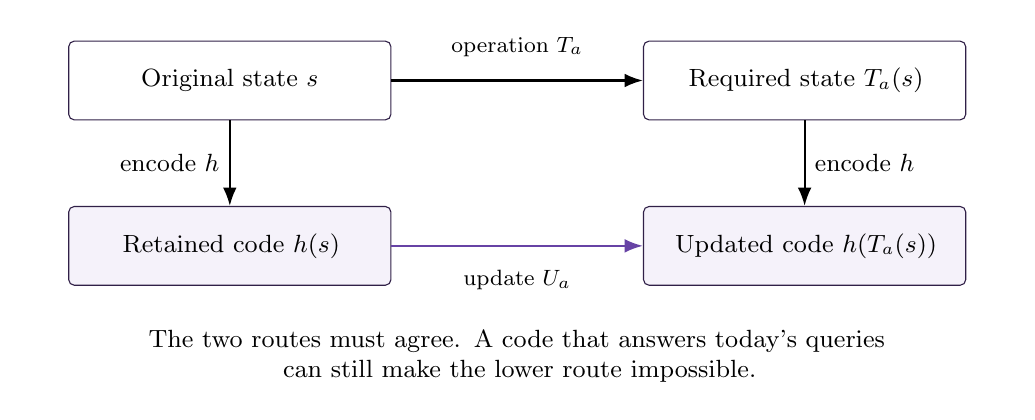
\begin{tikzpicture}[>=Latex,font=\small,box/.style={draw=ink,rounded corners=2pt,align=center,inner sep=7pt,minimum height=1.0cm}]
\node[box,text width=3.6cm] (s) at (0,0) {Original state $s$};
\node[box,text width=3.6cm] (t) at (7.3,0) {Required state $T_a(s)$};
\node[box,text width=3.6cm,fill=wash] (z) at (0,-2.1) {Retained code $h(s)$};
\node[box,text width=3.6cm,fill=wash] (u) at (7.3,-2.1) {Updated code $h(T_a(s))$};
\draw[->,thick] (s)--node[above=5pt,font=\footnotesize]{operation $T_a$}(t);
\draw[->,thick] (s)--node[left]{encode $h$}(z);
\draw[->,thick] (t)--node[right]{encode $h$}(u);
\draw[->,thick,draw=accent] (z)--node[below=5pt,font=\footnotesize]{update $U_a$}(u);
\node[align=center,text width=12.2cm] at (3.65,-3.5) {The two routes must agree. A code that answers today's queries\\can still make the lower route impossible.};
\end{tikzpicture}
\caption{An executable abstraction must preserve operations as well as answers. The lower route has no access to the actual original state. The equality is checked for every modeled state and operation, then extends to arbitrary finite operation sequences by induction.}\label{fig:square}
\end{figure}

\section{Construct the distinctions that the purpose requires}
\label{sec:conflict}
\subsection{Static answerability is a coloring problem}
Two states conflict if one admissible context would require different answers from them:
\begin{equation}
\{s,t\}\in E_0\ \Longleftrightarrow\ \exists c:\ s,t\in D_c,\quad f_c(s)\ne f_c(t).\label{eq:conflict}
\end{equation}
Let $G_0=(\Sset,E_0)$. A code admits a correct static decoder exactly when it assigns different labels to the endpoints of every edge. The minimum static alphabet is therefore $\chi(G_0)$, the graph's chromatic number.

The proof is direct. A conflicting pair cannot share one label because the decoder sees the same label and context. Conversely, all states sharing a label and an admissible context have one required answer, so the decoder can return it. This is the characteristic-graph logic of functional compression, not a new coding theorem \citep{orlitsky,doshi}. Its practical use here is to turn a false merge into a concrete question on which it fails.

Compatibility need not be transitive. State A may be mergeable with B, and B with C, while A conflicts with C. There need not be one unique coarsest answer-preserving partition. A procedure that simply closes pairwise compatibility transitively can create an incorrect representation. Exact coloring chooses a globally compatible assignment instead.

\subsection{Let future operations generate new obligations}
For a word $w=a_1\cdots a_k$, let $T_w=T_{a_k}\circ\cdots\circ T_{a_1}$. Two original states may become distinguishable after $w$ even if they do not conflict now. Define
\begin{equation}
\{s,t\}\in E_\infty\ \Longleftrightarrow\ \exists w:\ \{T_w(s),T_w(t)\}\in E_0.\label{eq:future}
\end{equation}
The empty word is allowed. The compiler constructs this graph by repeatedly adding preimages of existing conflicts under each operation. It terminates because there are at most $\binom{|\Sset|}{2}$ unordered pairs. With each added pair it retains an operation word and terminal context witnessing the required distinction.

\begin{proposition}[Frozen-code sufficiency with external history]\label{prop:history}
A code $h$ permits correct answers from $(h(s),w,c)$ for every admissible future query after every finite word $w$ if and only if $h$ properly colors $G_\infty$.
\end{proposition}
\begin{proof}
An edge of $G_\infty$ supplies a word and context that make two identically encoded states require different answers, proving necessity. If the code is proper, every original state with the same label whose transformed state lies in $D_c$ has the same required answer after $w$. Returning that answer proves sufficiency. Empty compatible sets are rejected rather than assigned an answer.
\end{proof}

This proposition deliberately gives the decoder the external operation word. It does not supply an update function. A proper coloring of $G_\infty$ can map two same-colored states into different colors after the same operation. The code can then answer with a sufficiently rich history, but cannot update itself from its own present label.

\begin{proposition}[Executable-code criterion]\label{prop:executable}
A proper coloring $h$ of $G_0$ admits canonical updates if and only if
\begin{equation}
 h(s)=h(t)\ \Longrightarrow\ h(T_a(s))=h(T_a(t))\quad\text{for all }s,t,a.\label{eq:congruence}
\end{equation}
Every such code is a proper coloring of $G_\infty$.
\end{proposition}
\begin{proof}
A deterministic $U_a$ must give one successor label to each current label, so Equation~\eqref{eq:congruence} is necessary. If it holds, define $U_a(z)$ from any representative of the nonempty fiber $h^{-1}(z)$; it is well defined. Induction on a word preserves equality of labels. A future conflicting pair therefore could not have shared its initial label.
\end{proof}

Closure and transition consistency are familiar state-minimization requirements \citep{kam,pena,givan}. The paper's constructor uses them operationally: it emits either a checked code or a pair of source states that share a proposed code but demand different updates. It does not replace a failed update proof with agreement among language-model critics.

\section{An exact constructor from the cycles of reasoning}
\label{sec:orbit}
The general optimization can be expensive. The reference can exhaustively search canonical partitions for small finite systems. The more useful construction below exploits a specific structural class and proves exactly when it is sufficient.

Let the single permitted operation $\tau$ be a permutation of $\Sset$. Its cycles are called orbits. Future closure makes $G_\infty$ invariant under this permutation. Suppose every orbit induces a clique. Suppose also that between any two orbits of the same length, all cross pairs conflict or none do. Partial, phase-sensitive interactions are excluded from this specialized constructor.

For each orbit length $\ell$, form an orbit-conflict graph $J_\ell$: one vertex per length-$\ell$ orbit, with an edge when their cross relation is complete. Relations between different orbit lengths need not be uniform.

\begin{theorem}[Orbit-wise executable representation]\label{thm:orbit}
Under these assumptions, the minimum canonical executable alphabet is
\begin{equation}
\boxed{\quad M_{\rm exec}=\sum_{\ell}\ell\,\chi(J_\ell).\quad}\label{eq:orbit}
\end{equation}
An attaining encoder and update function can be constructed from minimum colorings of the $J_\ell$.
\end{theorem}
\begin{proof}
An orbit of length $\ell$ is a clique, so its states receive $\ell$ distinct labels. Transition consistency makes those labels a cycle of the update function with exact period $\ell$. Two update cycles sharing a label are the same cycle, hence have the same length. Source orbits of different lengths therefore cannot share any label.

For one length, two orbits with a complete cross conflict cannot share an update cycle. Assigning each orbit its update-cycle identity consequently gives a proper coloring of $J_\ell$. At least $\chi(J_\ell)$ disjoint length-$\ell$ cycles are required, yielding the lower bound.

Conversely, give each color of a minimum coloring of $J_\ell$ one new cycle of $\ell$ labels. Map every source orbit of that color to this cycle in its permutation order. Uniform empty cross relations permit any phase alignment; complete ones have different colors. Use disjoint labels for different lengths. Rotating the code cycle realizes $\tau$, and no conflicting pair is merged. Static decoding follows from properness. The number of labels is exactly Equation~\eqref{eq:orbit}.
\end{proof}

The theorem is a concrete specialization, not a polynomial solution to arbitrary machine minimization. Exact coloring of the orbit graphs can still be hard. Its advantage is constructive: where the assumptions hold, it replaces a search over all source partitions with colorings of smaller orbit graphs and returns executable operations, not merely a bound on code size.

\begin{algorithm}[htbp]\small
\caption{Construct a canonical reasoning interface: implemented orbit backend}\label{alg:compile}
\begin{algorithmic}[1]
\Require Source states; admissible contexts and answers; a permitted permutation
\State Build current answer conflicts and retain their separating contexts
\State Close conflicts under operation preimages; retain witness words
\State Decompose the permutation into source orbits
\State Check orbit cliques and uniform equal-length cross relations
\If{a structural premise fails}
  \State Return an explicit unsupported-class result, not an optimality claim
\EndIf
\For{each orbit length $\ell$}
  \State Construct $J_\ell$ and solve its finite coloring problem exactly
  \State Allocate one $\ell$-label cycle per color; map source phases to it
\EndFor
\State Construct all supported answer decoders and the label-update table
\State Separately check every context--state outcome and update equation
\State Return the code, decoder, updates, scope, and optimality evidence
\end{algorithmic}
\end{algorithm}

The generic implementation discovers the orbits from a transition table; they are not supplied as the desired answer. It does receive the complete finite states, transitions, context semantics, and output obligations. Natural-language formalization and acquisition of a correct world model are not performed by this experiment.

\section{The decisive construction: replace the representation, not the purpose}
\label{sec:retirement}
\subsection{A small language that answers correctly}
Let $p\ge5$ be an odd prime and let $s=(x,y)\in\mathbb Z_p^2$. Context $(a,b)$ promises
\begin{equation}
 x\in\{a,a+1\},\qquad y\in\{b,b+1\},\label{eq:context}
\end{equation}
with arithmetic modulo $p$. The answer must be the actual pair. The context is available to every decoder, not only to the new method.

The code
\begin{equation}
 h_0(x,y)=x+2y\pmod p\label{eq:old}
\end{equation}
answers every static query. Indeed, differences inside one context satisfy $\Delta x,\Delta y\in\{-1,0,1\}$; $\Delta x+2\Delta y$ is zero modulo $p\ge5$ only when both are zero. The four candidates in each context have distinct labels.

At $p=5$, the five-label code is optimal. The exact graph solver and a separately implemented independent-set search establish that its 25-vertex conflict graph has independence number five, implying at least five colors. The expression search examines every $ax+by\pmod5$ with $a,b\in\mathbb Z_5$; eight are valid, and the fixed lexicographic rule selects $(a,b)=(1,2)$. The winning coefficients are computed, while the modular expression grammar is supplied.

Two independently encoded coordinates instead require three labels each, because each coordinate's conflict graph is an odd cycle. Their joint alphabet has nine combinations. Joint encoding's five-versus-nine effect is the classical pentagon-product phenomenon associated with Shannon capacity \citep{shannon,lovasz}, reconstructed here as a transparent starting point. It is not our new theorem, and a distributed system must pay for whatever access permits the joint encoder to see both coordinates.

\subsection{One legitimate operation breaks the old thought}
Now permit
\begin{equation}
 \tau(x,y)=(gx,y),\label{eq:tau}
\end{equation}
where $g$ is a primitive root modulo $p$. A primitive root cycles through every nonzero residue. For $p=5$, choose $g=2$.

States $(0,0)$ and $(3,1)$ both have old label zero. Their successors are $(0,0)$ and $(1,1)$, which lie in the same context $\{0,1\}\times\{0,1\}$ but require different answers. No deterministic update of the old zero label can resolve that distinction. This is an information failure of the representation, not an incorrectly chosen confidence threshold.

Future conflicts are particularly simple. Repeated multiplication by $g$ can bring any nonzero first-coordinate difference to one. The second coordinate never changes. Consequently, two distinct states conflict under some continuation exactly when their second coordinates are equal or adjacent. For each fixed $y$ there is a $p$-state clique; neighboring $y$-rows are completely joined, and nonneighboring rows are not. In graph notation,
\begin{equation}
 G_\infty=K_p\boxtimes C_p=C_p[K_p].\label{eq:blowup}
\end{equation}
The equality is derived from the operation and context semantics, not stipulated as the desired graph.

\subsection{A smaller executable language}
There are $p$ fixed points $(0,y)$ and $p$ nonzero-$x$ orbits of length $p-1$, one for each $y$. Within either orbit-length class, the orbit-conflict graph is the odd cycle $C_p$, whose chromatic number is three. Theorem~\ref{thm:orbit} gives
\begin{equation}
 M_{\rm exec}=1\cdot3+(p-1)\cdot3=3p.\label{eq:3p}
\end{equation}

An explicit attaining code is
\begin{equation}
 h_1(x,y)=(x,\kappa(y)),\qquad
 \kappa(y)=\begin{cases}y\bmod2,&0\le y\le p-2,\\2,&y=p-1.\end{cases}\label{eq:new}
\end{equation}
The update is $(x,k)\mapsto(gx,k)$. Given the context, exactly one of its two adjacent $y$ values has color $k$, while $x$ is directly retained. The representation therefore answers the unchanged question and continues indefinitely through the declared operation without retaining its execution history. This is also the strong conventional reference: a specialist supplied with the same mathematics obtains the same minimum.

\begin{theorem}[Retiring an internal representation can be strictly cheaper]\label{thm:retire}
For the prime-family contract above, a canonical executable representation needs at least $3p$ labels, and Equation~\eqref{eq:new} attains this minimum. In contrast, any canonical executable representation $r$ from which the old label $h_0$ is recoverable without context needs at least $p^2$ labels.
\end{theorem}
\begin{proof}
The first statement follows from Theorem~\ref{thm:orbit}. For the second, suppose $h_0=\rho\circ r$ and $r\circ\tau=U\circ r$. From $r(x,y)$ one can compute both
\begin{equation}
 u=\rho(r(x,y))=x+2y,\qquad
 v=\rho(U(r(x,y)))=gx+2y.
\end{equation}
Since $g-1$ and 2 are invertible modulo $p$,
\begin{equation}
 x=(g-1)^{-1}(v-u),\qquad y=2^{-1}(u-x).\label{eq:recover}
\end{equation}
Thus $r$ distinguishes every original state and has at least $p^2$ labels. Full-state retention attains that refinement bound.
\end{proof}

The separation in alphabet size is $p/3$ and grows with the declared family. In fixed-length bits it compares $\bits{p^2}$ with $\bits{3p}$, not an unbounded ratio of intelligence or inference speed. The discarded object is an internal label, not a required fact. If recovering $h_0$ without context becomes a genuine output obligation, the $p^2$ lower bound is the correct requirement, not a defect to hide.

\begin{figure}[htbp]\centering
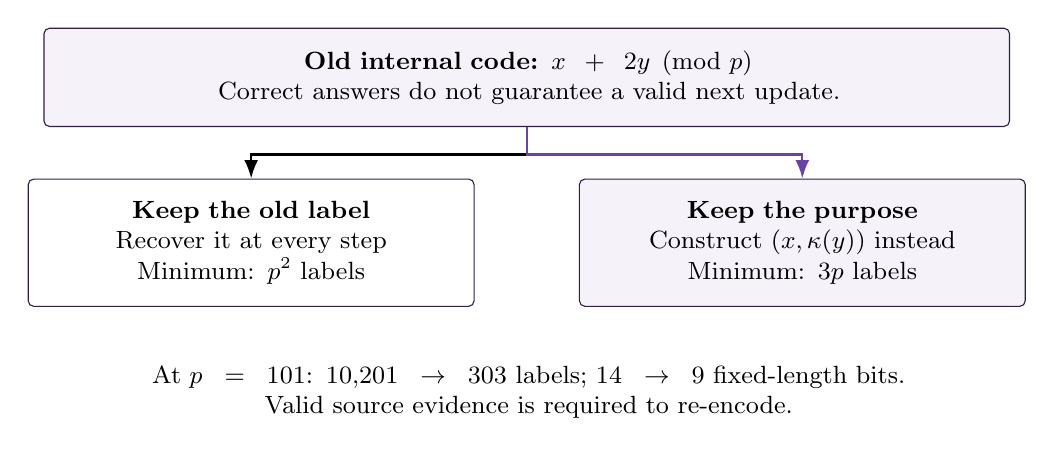
\begin{tikzpicture}[>=Latex,font=\small,box/.style={draw=ink,rounded corners=2pt,align=center,inner sep=8pt}]
\node[box,fill=wash,text width=11.7cm] (old) at (0,0) {\textbf{Old internal code:} $x+2y\pmod p$\\Correct answers do not guarantee a valid next update.};
\node[box,text width=5.1cm,minimum height=1.5cm] (keep) at (-3.5,-2.1) {\textbf{Keep the old label}\\Recover it at every step\\Minimum: $p^2$ labels};
\node[box,fill=wash,text width=5.1cm,minimum height=1.5cm] (replace) at (3.5,-2.1) {\textbf{Keep the purpose}\\Construct $(x,\kappa(y))$ instead\\Minimum: $3p$ labels};
\draw[->,thick] (old.south)--++(0,-.35)-|(keep.north);
\draw[->,thick,draw=accent] (old.south)--++(0,-.35)-|(replace.north);
\node[align=center,text width=12.2cm] at (0,-4.0) {At $p=101$: $10{,}201\to303$ labels; $14\to9$ fixed-length bits.\\Valid source evidence is required to re-encode.};
\end{tikzpicture}
\caption{The advantage comes from retiring an unnecessary internal constraint. Both final interfaces face the same answers, contextual information, and operation. One additionally preserves the predecessor's internal code. The new code is not computed from the old label alone.}\label{fig:retire}
\end{figure}

\subsection{Retirement does not manufacture lost information}
The new code distinguishes states that the old code merged. There is no function mapping the old label alone to the new code in general. Re-encoding must use retained source data, an independently sufficient earlier context and history, or genuinely new information. The portable experiment initializes each code from the actual supplied source. It does not pretend that a discarded source can be recovered from a clever instruction.

This separates two assets for \Om: an authoritative evidence archive and a compact active reasoning representation. An archive can enable later recompilation, but its storage, access, and revalidation are real costs. The resident-label theorem does not imply that keeping an uncompressed archive somewhere else consumes no memory. After deliberate source erasure, some future amendments must be refused.

\section{Answerable is not yet executable}
\label{sec:gap}
\subsection{Thirteen labels with history, fifteen without it}
For the 25-state successor at $p=5$, $G_\infty$ is a five-cycle of five-vertex cliques. An independent set contains at most two vertices: at most one per row, and at most two nonadjacent rows. Hence any static code for the closed graph needs at least $\lceil25/2\rceil=13$ labels. The companion constructs twelve independent pairs and one singleton, attaining thirteen.

That code can answer after any number of operations when supplied its original label and the operation exponent modulo four. The study checks all four exponents against every admissible context--state case. But it cannot update its label from the label alone. The canonical executable minimum is fifteen, established by the orbit theorem.

These are different resource accounts. Thirteen labels alone and fifteen labels alone both fit in four bits. Thirteen source labels \emph{plus} an externally retained four-valued exponent allow 52 pairs, requiring six bits under a joint fixed-length count. Calling the history-assisted design a thirteen-state recurrent implementation would conceal a carrier of information.

\begin{table}[htbp]\centering\small
\caption{Exact distinctions in the $p=5$ construction. ``Static'' can answer supported queries; ``canonical'' also updates its current code without source re-access or external operation history.}\label{tab:frontier}
\begin{tabularx}{\linewidth}{@{}YrY@{}}\toprule
Representation & Labels & Continuing capability\\\midrule
Old joint static code & 5 & Correct before the new operation; invalid afterward\\
Code for all future conflicts & 13 & Correct with external operation history\\
Minimum canonical executable code & 15 & Correct answers and in-place updates\\
Static correction appended to old code & 15 & Correct static successor answers; tested code is not updateable\\
Executable refinement preserving old label & 25 & Retains more internal information than the purpose needs\\\bottomrule
\end{tabularx}
\end{table}

\subsection{A three-bit obstruction}
A smaller variation makes the bit distinction sharp. Take $x\in\mathbb Z_3$, $y\in\mathbb Z_5$, the same adjacent-pair contexts, and $\tau(x,y)=(2x,y)$. The conflict graph is $C_5[K_3]$ and is already operation-invariant. Its independence number is two. Eight labels suffice by an independent-pair cover, and fewer cannot cover fifteen vertices. The orbit theorem instead requires
\begin{equation}
 1\cdot\chi(C_5)+2\cdot\chi(C_5)=9
\end{equation}
labels for a canonical executable representation.

\insight{\textbf{Three bits can preserve enough information to answer every current query. No three-bit canonical representation can also perform the declared update.}\par\smallskip The missing capacity is not another answer. It is an executable continuation.}

Canonical encoding is a substantive restriction. Our bound does not rule out more general history-dependent compatible-state assignments. This distinction matters in both incomplete-machine minimization and recent recurrent-memory work \citep{pena,li2026}. We do not relabel the present alphabet minimum as a universal lower bound on every possible agent memory architecture.

\subsection{Appending information is a different optimization problem}
Suppose a static code $h$ must remain part of a message while the answer-conflict graph changes to $G'$. If an extra label $e(s)$ may depend on the original source, then the minimum extra alphabet is
\begin{equation}
 M_{\rm extra}=\max_{z\in h(\Sset)}\chi\bigl(G'[h^{-1}(z)]\bigr).\label{eq:extension}
\end{equation}
Each old fiber needs a proper coloring of its induced new conflicts. Extra labels can be reused across different old fibers because the decoder sees the old label too. The minimum number of actually used combined labels is the sum of these chromatic numbers. This elementary static result carries no transition guarantee.

In the anchor, each five-state old fiber requires three correction labels. Fifteen combined labels suffice for static successor answers. The emitted correction nevertheless fails the update test. If the old label must remain recoverable \emph{at every current state}, transition-stable refinement reaches all twenty-five states, as Theorem~\ref{thm:retire} requires. Equal alphabet counts do not establish equal capabilities.

\section{What the executable study actually establishes}
\label{sec:study}
The reference uses Python's standard library, exact finite relations, integer arithmetic, and JSON artifacts. It makes no language-model call. Source states, operation tables, context validity, output semantics, and the candidate expression grammar are supplied. The program constructs graphs, closure witnesses, colorings, orbit codes, update functions, decoders, and refinement failures. It does not autonomously discover a physical world or the semantics of a customer's task.

\subsection{A generic constructor and a strong unrestricted reference}
The orbit backend reads arbitrary finite transition tables, discovers their cycles, tests its structural premises, and colors the resulting orbit graphs. A separate reference enumerates all canonical set partitions and directly checks the original context outputs and transitions. It does not call the conflict constructor or the orbit theorem implementation.

Across eighty source-bound generated models with permuted state labels, the two implementations agree on every minimum. The reference examines 26,912 partitions. These cases have varied orbit lengths, cross conflicts, and state numbering; they are author-selected software checks, not independent scientific discoveries. Every unrestricted reference has the same permitted source and transition information.

Forty additional general finite systems have one or two total operations, including nonpermutations. Their conflict closure and witness generation are checked, and exhaustive canonical partition search constructs their valid codes. The reference examines another 11,470 partitions. These cases do not establish that the orbit backend handles nonpermutations: its corresponding restriction remains enforced.

\subsection{Exact coverage of the static subsolver}
The graph-coloring subsolver is checked on every labeled simple graph with one through five vertices: $1+2+8+64+1024=1,099$ graphs. A separately implemented set-partition reference tests the original pairwise answer requirements. All minimum color counts agree across 54,253 reference partitions.

The 25-state anchor additionally uses a separate independent-set search to establish the lower bound of five. The finite expression search tries all twenty-five coefficient pairs and retains failures as well as its eight valid candidates. Its selected modular code ties the exact unrestricted coloring optimum. No comparison claims that a competent coding-theory specialist would fail to construct it.

\subsection{The prime family is checked as a family}
For $p\in\{5,7,11,17,31,101\}$, the driver generates all $p^2$ source states, all adjacent-pair contexts, the primitive-root operation, and the explicit minimum replacement interface. Every admissible outcome and every update equation is checked. Equation~\eqref{eq:recover} is independently evaluated for every source state to check the preservation obstruction's arithmetic.

\begin{table}[htbp]\centering\small
\caption{Executed prime-family checks. The exact minimum formulas are proved; the software checks every represented source and admissible query. Large cases use the explicit symbolic specialization, not exhaustive partition search.}\label{tab:primes}
\begin{tabular}{@{}rrrrrr@{}}\toprule
$p$ & Preserving & Replacement & Keep & Replace & Query checks\\
 & labels & labels & bits & bits & \\\midrule
5 & 25 & 15 & 5 & 4 & 100\\
7 & 49 & 21 & 6 & 5 & 196\\
11 & 121 & 33 & 7 & 6 & 484\\
17 & 289 & 51 & 9 & 6 & 1,156\\
31 & 961 & 93 & 10 & 7 & 3,844\\
101 & 10,201 & 303 & 14 & 9 & 40,804\\\midrule
Total & 11,646 & & & & 46,584\\\bottomrule
\end{tabular}
\end{table}

The $p$-label initial code is proved valid throughout this family. It is proved minimum only for the five-by-five anchor; the paper does not assume that it is the best static representation at every larger prime. The retirement theorem concerns the cost of preserving this specific inherited code, not every possible predecessor code.

\subsection{An actual portable reasoning interface}
The fifteen-label dynamic anchor is serialized with its model identity, code map, decoder tables, update table, and an explicit false authority flag. A separately loaded reader checks its checksum and reconstructs its semantic tables before admitting it. The resulting artifact is executable data, not a proposed interface illustration.

For each of the twenty-five source states, the experiment performs twenty consecutive updates. At every step it selects an admissible context and checks the decoded state against the direct source transition. All five hundred update/query steps agree. The reader advances its label without receiving the actual source state; the driver retains source truth only for evaluation.

The same frozen interface supports two new supplied output adapters: a target label $(x+3y)\bmod5$ and the least-cost action $j\in\{0,\ldots,4\}$ under
\begin{equation}
 (j-x)^2+(4-j-y)^2.
\end{equation}
All one hundred admissible context--state cases agree with direct calculations. These tasks have a different output and optimization rule, but follow trivially from a successfully reconstructed state. They demonstrate usable downstream composition, not autonomous discovery, cross-industry transfer, or a newly learned reasoning policy. The common core is unchanged; the new adapters are not free constructions in a commercial cost account.

\subsection{A payload study, not a claim about intelligence}
A separate experiment encodes thirty-two five-valued coordinates in sixteen pairs, using the static joint modular code and the same contextual information for all methods. All 4,096 seeded trials decode correctly. Independent three-label coordinate encodings have $3^{32}$ possible payloads and need 51 globally packed fixed-length bits; paired encodings have $5^{16}$ payloads and need 38. If each small field is stored separately, the comparison is 64 versus 48 bits.

This is an encoded-payload count. It omits neither by implication nor by magic the cost of contexts, codebooks, compilation, data movement, or the joint encoder's access. It is not an observed language-model token saving, shorter chain of thought, or runtime speedup. It illustrates the classical joint-coding mechanism, not the main representation-retirement contribution.

\begin{table}[htbp]\centering\small
\caption{Completed evidence, with units kept separate. The checker and constructor share authorship; no external institutional validation is claimed.}\label{tab:evidence}
\begin{tabularx}{\linewidth}{@{}YrY@{}}\toprule
Check & Count & Evidential meaning\\\midrule
All simple conflict graphs of sizes 1--5 & 1,099 & Exact static minima agree with partition reference\\
Generated orbit-model comparisons & 80 & Exact executable minima agree with unrestricted reference\\
General finite-system comparisons & 40 & Closure witnesses and canonical reference codes checked\\
Prime-family context--state checks & 46,584 & All supported outcomes in six specified instances\\
Prime-family transition checks & 11,646 & Every source update commutes with its code\\
Portable continuation steps & 500 & Actual data-only reader updates and answers\\
Fresh supplied adapter cases & 100 & Unchanged core supports both new output adapters\\
Static batch trials & 4,096 & Payload decoding, not discovery or model benchmarking\\
Unit-test methods & 44 & Functional, boundary, and tampering tests\\\bottomrule
\end{tabularx}
\end{table}

\section{Three failures that a useful reasoner must preserve}
\label{sec:failures}
\subsection{A false context can make a checked answer wrong}
The semantic certificate assumes that the context is true. In the executed negative control, the actual state is $(0,0)$, while the supplied second-coordinate context falsely says $y\in\{1,2\}$. The retained cycle color is also compatible with $y=2$. The valid decoder therefore reports $(0,2)$ under that false premise.

Some inconsistent contexts are rejected because no encoded state supports them. This control shows why not all false contexts are detectable. Hashes authenticate artifact bytes, not observations. Exact finite decoding does not certify a sensor, an extracted fact, or an omitted real-world state. A natural application needs a separately justified model and evidence-to-context bridge.

\subsection{A second operation can erase the compression advantage}
Add the independent operation $(x,y)\mapsto(x,2y)$ to the $p=5$ model. Repeated coordinate multiplications can bring every nonzero coordinate difference to one. The future conflict graph becomes the complete graph on twenty-five states, so every static future-safe code---and therefore every executable one---requires all twenty-five labels. The driver constructs all 300 edges after two closure rounds.

The correct response is not to defend a permanent compression ratio. The supported operation family changed. A compact representation is a capability under a contract, not a promise to answer every future question under every future transformation. This is why the capsule includes its actual operation semantics and why adding an operation requires requalification.

\subsection{Orbit structure can be insufficient}
Two equal-length orbits can have a phase-sensitive cross relation: some aligned pairs conflict and others do not. The theorem's complete-or-empty premise then fails. Sharing an update cycle may be possible only at a particular phase, or may be impossible. The implemented specialized constructor refuses such cases. Treating any conflict as complete can lose the optimum; ignoring it can produce wrong answers.

More general machines may need a different exact search, a justified approximation, or a richer compatible-cover representation. The small exhaustive reference supplies a correct canonical answer where feasible, not a scalable replacement for those literatures. General graph coloring and finite-state minimization do not become easy because the output is called a thought.

\section{What is new, and what belongs to established theory?}
\label{sec:prior}
The most important distinction is not between a fashionable name and an old algorithm. It is between a clearly scoped construction and an unsupported claim of general reasoning superiority.

Characteristic-graph coding already connects required functional outputs with permissible source merging \citep{orlitsky,doshi}. Shannon and Lovász supply the classical pentagon neighborhood of the static example \citep{shannon,lovasz}. Incompletely specified finite-state minimization already requires compatible outputs and valid transitions, including models richer than disjoint canonical partitions \citep{kam,pena}. We use these precedents rather than claiming that answer sufficiency or transition closure began here.

The narrower mathematical center is Equation~\eqref{eq:orbit}, its explicit constructor, and the retirement family in Theorem~\ref{thm:retire}. The former identifies a solvable orbit-structured subclass. The latter proves that retaining a particular previously useful internal label can impose a strictly larger minimum than preserving the underlying task. This targeted review does not establish that no related group-action or automata result exists elsewhere; broader novelty remains subject to specialist review.

\begin{table}[htbp]\centering\small
\caption{Closest antecedents and the actual scope of the present result. None of the named systems was benchmarked here.}\label{tab:prior}
\begin{tabularx}{\linewidth}{@{}P{.24\linewidth}YY@{}}\toprule
Foundation & Established question & Present specialization\\\midrule
Functional compression & What distinctions does a decoder need for a function with side information? & Derive current and future conflicts from a supplied reasoning contract\\
Incomplete-machine minimization & Which compatible states can share a closed implementation? & Exact canonical code for clique orbits with uniform interactions\\
Knowledge compilation & How do compact languages trade off query and transformation support? & Construct an encoder, decoder, and actual update table together\\
Recurrent behavioral memory & What must be retained to reproduce behavior through future observations? & Worst-case finite alphabet and a specific old-label retirement separation\\
Learned latent reasoning & Can learned internal states support more effective model reasoning? & No neural learning; inspectable finite semantics and exact certificates\\\bottomrule
\end{tabularx}
\end{table}

\citet{li2026} is a close contemporary comparison: it separates instantaneous from recurrent behavioral requirements and treats more general closed compatible assignments. Its behavioral and learned-memory results must not be attributed to this paper. We instead analyze deterministic canonical codes under supplied operations and expose the cost of preserving a designated old code. These are different optimization models; their minima are not interchangeable.

\citet{darwiche} already makes representation choice answer to both query and transformation support. Our finite commutation condition is one concrete way to make that requirement executable. Value-preserving model minimization likewise provides the background for retaining only distinctions relevant to continued behavior \citep{givan}. The word ``transformational'' refers to making the representation editable while preserving the external purpose; it is not evidence that ordinary abstraction theory is inadequate.

\section{Where current AI can contribute}
\label{sec:ai}
The research cutoff is 21 October 2026. Current work supplies proposal mechanisms and strong comparison families, not a completed natural-language-to-proof pipeline for the present compiler.

DreamCoder learns reusable program abstractions \citep{dreamcoder}. Coconut studies learned reasoning in a continuous latent space \citep{coconut}. GEPA and Automated Design of Agentic Systems optimize prompts or agent implementations using feedback \citep{gepa,adas}. AlphaEvolve generates and evaluates executable program candidates \citep{alphaevolve}. These approaches could propose task formalizations, compact encodings, or implementations of an update rule. They could also find a better construction than the one in this manuscript.

What the reference adds is an inspectable obligation: a candidate representation must preserve every declared answer and commute with every admitted update. A model-generated explanation of why its abstraction is good does not discharge those obligations. Conversely, a representation found by a conventional solver is not less useful because it was not produced by a language model.

A future model experiment should hold model version and access, initial evidence, permitted tools, total search effort, and human intervention comparable. Every competitor must be allowed to change the representation and to use established synthesis tools. Separate the ability to discover a valid contract from the ability to solve a supplied one. Then freeze proposed code, operations, and confirmation tasks before fresh tests. A larger inherited archive is an additional asset, not proof of a better discovery policy.

Computer use can expose software and obtain permitted inputs; it does not determine the sufficient reasoning representation. A validated programmatic interface can be better than repeatedly interpreting a screen. No current professional-job automation rate or broad labor-market estimate is used to support the present result. The executed contribution remains mathematical compilation, not a frontier-model performance claim.

\section{A concrete SUCCESSOR \texorpdfstring{$\Omega$}{Omega} increment}
\label{sec:successor}
The implementation target is \href{https://github.com/MontrealAI/AGI-Alpha-Agent-v0}{AGI Alpha Agent / SUCCESSOR $\Omega$}. The proposed addition is a \emph{reasoning-interface record}, attached to the existing project history rather than a parallel platform. Its fields are the supported source semantics, context premises, questions, operations, encoder, decoder, update rules, witnesses, and invalidation conditions. The companion implements the local finite core and portable reader; production integration is not claimed.

A useful interface should distinguish four outcomes: \emph{answer supported}; \emph{current answer supported but continuation unsupported}; \emph{new representation required}; and \emph{source evidence insufficient for recoding}. These outcomes tell a user what is missing. They should not be collapsed into one confidence score or a badge inherited from an earlier success.

The strongest successor behavior is selective retirement. It retains the evidence and the externally meaningful accomplishments while replacing an internal scheme that no longer serves the new operation. The archive records what changed, why the old representation failed, what was paid to reconstruct the new one, and which obligations still hold. Historical success remains true; its scope is not retroactively expanded.

The pipeline connects the research sequence without conflating its results. Out-Think constructs a supported internal language. Out-Strategise can use it to choose what to observe or build. Out-Execute can retain artifacts and commit supported effects safely. Each stage requires its own actual adapter, permissions, and outcome validation. Combining their names is not evidence that the integrated system already works.

\subsection{A first natural research campaign}
Select a benign, externally specified software-analysis or scientific-decision workflow with recurring contextual queries and real state transformations. Establish the original full-state reference, the required outputs, the source of contextual facts, and the permitted updates. Ask competing systems to construct a smaller useful interface without supplying the winning representation.

An admissible result must explain both the proposed merges and their continuations. Tests should include a context change, a new operation, a false contextual premise, an old internal quantity that becomes unnecessarily expensive to preserve, and a case where the full representation is preferable. Measure construction, integration, decoding, updates, source retention, and requalification separately. A live-model campaign and domain deployment remain future work; neither is inferred from the exact finite checks.

\section{Invent the economy around the capability, not around more thinking}
\label{sec:economy}
\emph{Invent the Economy} treats the capability, beneficiary, acceptance terms, rights, financing, and delivery arrangement as a joint construction \citep{boucherEconomy}. Here the technical variable is explicit: which internal representation supports a customer's actual questions and operations at a useful complete cost. The commercial unit should be a qualified reasoning interface, not a promise to generate more intermediate tokens.

A prospective customer could commission a bounded investigation into an expensive recurring software or scientific workflow. The research deliverable would include a credible reference, proposed abstraction, executable decoder and update rules, failure witnesses, and a decision about deployment. A valid negative finding can complete that research scope. Actual deployment requires an accepted interface whose context premises and state semantics are justified in the customer's environment.

The arrangement can change the technical problem. Requiring every historical internal label as an output forces a refinement contract. Requiring only the real decision outcomes can permit a smaller replacement. That distinction must be negotiated honestly: a material audit or traceability obligation cannot be deleted merely because it makes the abstraction larger. Likewise, an architecture that supplies trusted context can enable a compact interface, while acquiring that context may cost more than keeping the raw state.

A derived lifecycle comparison is
\begin{equation}
 C_{\rm construct}+C_{\rm qualify}+C_{\rm migrate}
 +\sum_{j=1}^{N}\bigl(C_{{\rm update},j}+C_{{\rm decode},j}+C_{{\rm context},j}\bigr)
 +C_{\rm archive}+C_{\rm maintain}<C_{\rm alternative}.\label{eq:economy}
\end{equation}
Both sides must deliver the same required outcomes over the same horizon. The alphabet theorem supplies one design constraint, not monetary values for this inequality. The tiny reference instances do not establish material storage savings or willingness to pay. Fixed codebooks and validation can overwhelm their payload savings.

A shared constructor may support multiple applications, but each needs valid semantics, adaptation, accepted terms, and delivery economics. Reusing one finite decoder under two supplied output functions is technical composition, not two businesses. Sponsors, customers, prices, and revenues are not invented in this manuscript. Future receipts do not finance earlier construction without usable authorized funding; advances retain their actual obligations and refund exposure.

MONTREAL.AI's parent ownership remains intact. Reusable implementations and evidence can be retained only under applicable licenses and actual agreements. Public coding theory does not create exclusive rights by appearing in a registry. Qualified delivery, integration, maintenance, and continued useful construction would need to justify commercial value against copying and stronger competitors.

The inherited project distinguishes AGIJobManager's USDC route from the Alpha / Jobs v0 \$AGIALPHA routes \citep{boucherEconomy,boucherExecute}. This paper changes no asset, contract, fee, holder right, or operational permission. A useful reasoning service can create customer value without creating token-holder equity, dividends, or a determinate token price. Eliminating unnecessary thinking should be permitted to reduce billed activity rather than generate artificial work to preserve fees.

The larger productive pathway remains evidence-dependent: a useful representation supports accepted applications; legitimate receipts after obligations fund another capability; that capability may make a more consequential scientific or productive undertaking possible. Context acquisition, formalization, engineering, integration, finance, and physical limits can interrupt that sequence. The paper contributes one constructible means of improving a reasoning interface, not a forecast of inevitable expansion.

\section{Conclusion: preserve the capability, not the shape of the old thought}
A correct answer is not necessarily a sufficient state for what comes next. A representation can satisfy every present query, fail under one authorized operation, and become needlessly expensive if a successor is required to preserve its internal language. Adding more detail is then not the only legitimate move.

Out-Think makes the alternative explicit. The task generates current conflicts. Operations generate future distinctions. A supported orbit structure generates an exact executable code. The prime family proves when replacing a valid old code is strictly smaller than preserving and refining it, while a portable implementation checks answers and updates together. The same analysis exposes when extra operations remove the advantage and when a false contextual premise defeats an otherwise correct decoder.

The contribution is bounded, but the research target is substantial: intelligence that can construct the representations through which its next reasoning becomes possible, rather than treating every inherited internal distinction as permanent. A new language earns its place by the truths and operations it preserves, not by how sophisticated it sounds.

\insight{\textbf{Do not merely improve the next answer. Construct a better way for reasoning to continue.}\par\smallskip Preserve the purpose. Expose the missing distinction. Retire the representation that has become the restriction.}

\Needspace{11\baselineskip}
\section*{Research status}
This AI-assisted manuscript reports mathematical derivations, exact synthetic finite studies, and a portable data-only reasoning interface. The constructor and separate checker share authorship; no external peer review is claimed. The proofs are written mathematical arguments, not proof-assistant formalizations. No live-model discovery campaign, physical experiment, real customer acceptance, revenue, token-price study, or repository integration was performed. The current contribution is a canonical representation construction and its scoped comparisons, not general transformational intelligence. Earlier papers and remote systems remain unchanged.

\par\bigskip
\appendix
\section{Additional proofs and construction details}
\label{app:proof}
\subsection{Why preimage closure is complete}
Write $E_k$ for conflicts witnessed by a word of length at most $k$. At $k=0$, this is exactly Equation~\eqref{eq:conflict}. If a pair maps under operation $a$ into an edge witnessed by $w$, the original pair is witnessed by $aw$. Conversely, a nonempty witness word has a first operation and a suffix, so its pair appears under the corresponding preimage step. Induction proves equality with the iterative construction. Once no edge is added, every longer word is already covered. The finite pair set ensures termination.

The implementation stores each witness as an operation-index tuple and a context index. A separate test applies that word to the two source states and checks that both transformed states are admitted to the terminal context and have different required outputs. This is a finite semantic certificate, not evidence that a physical operation or extracted context is truthful.

\subsection{The exact eight- and thirteen-label static constructions}
Consider $C_5[K_p]$ with odd $p$. Each of five rows contains $p$ mutually conflicting states. Any two states in nonadjacent rows are compatible. Order the rows as $0,2,4,1,3$, so consecutive rows in this order are nonadjacent in the original cycle.

Let $p=2a+1$. Along the five edges of that reordered cycle, pair unused row vertices with counts $a,a+1,a,a+1,a$. Every row except the first uses all $p$ vertices; the first leaves one. Give each pair one code and the remaining vertex one code. This uses $(5p+1)/2$ labels. No independent set has more than two vertices, proving the matching lower bound $\lceil5p/2\rceil$. At $p=3$ and $p=5$ the values are eight and thirteen.

This is a static code. The constructed pairs do not generally map to pairs with the same successor label. The companion explicitly reports the conflicting updates, rather than assuming that an optimal static cover is automatically a state machine.

\subsection{Independent versus joint encoding}
For one five-valued coordinate whose context names an adjacent pair, each cycle edge must receive different labels. Two labels cannot color an odd cycle, and three suffice. If two encoders operate separately on $x$ and $y$, each must satisfy this requirement: fix the other coordinate and its valid context to see that a collision at either source is fatal. Since all source pairs occur, the combined alphabet has at least $3\cdot3=9$ messages. A joint encoder can use Equation~\eqref{eq:old} with five.

For completeness, the five-by-five graph's independence number has an elementary bound. Each row can contain at most two independent vertices. If a row contains two, their closed neighborhoods cover all five first-coordinate values, so both adjacent rows must be empty. The two other rows are adjacent to each other and can contain at most two vertices in total, giving at most four overall. If no row contains two, there are at most five vertices. The five states $(x,y)=(-2y,y)$ attain five. Thus the static coloring needs at least $25/5=5$ labels, independently of the exhaustive software check.

This argument has a strict access premise. A joint encoder receives both coordinates. An architecture that begins with distributed sources must count communication or colocated processing needed to make that possible. The five-label result does not establish a free distributed protocol with two isolated encoders.

\subsection{What retaining an old label really requires}
The refinement theorem assumes that a fixed map $\rho$ can recover $h_0$ from the \emph{current} new code. Merely retaining one historical old label beside a separate evolving state is a different design and must count both memories. The theorem also assumes canonical updates that realize the same source transformation. Neither condition can be dropped from its lower-bound statement.

A static refinement of an old partition can be made transition-stable by repeatedly replacing a label with the tuple of that label and the successor labels under all actions. Every iteration refines the old partition; when no class splits, Equation~\eqref{eq:congruence} holds. This is standard partition refinement. In the anchor it reaches twenty-five singleton classes. The orbit constructor instead searches a new partition that need not refine the old one and reaches fifteen. It changes the abstraction rather than merely completing its missing fields.

\subsection{Why additional operations can force identity}
With independent primitive-root multiplications on both coordinates, any nonzero difference in either coordinate can be brought to one, independently. For any distinct source pair, select exponents that make each nonzero difference adjacent and leave each zero difference equal. The transformed pair shares one adjacent-pair context and requires different answers. Thus every pair is an edge of future closure, proving the complete-graph lower bound. This is an information consequence of the enlarged operation family, not a failed implementation of the smaller code.

\section{Reproduction, custody, and complete resource accounting}
\label{app:reproduce}
The reference requires only Python's standard library. The recorded environment is Python 3.13.5 on Linux. There are no model-provider credentials, numerical-library dependencies, wallet calls, or external operations. The complete driver recorded approximately 0.323 seconds in the preparation run, excluding source authoring, mathematical work, research, review, rendering, and integration. This descriptive run time is not a comparison with a language model or an optimized compiler.

\begin{lstlisting}
python -S code/run_study.py
python -S -m unittest discover -s tests -v
python -S code/query_interface.py results/reasoning_interface.json \
  --state 16 --steps 1 --context 0
xelatex -no-shell-escape -interaction=nonstopmode \
  -halt-on-error Out_Think.tex
xelatex -no-shell-escape -interaction=nonstopmode \
  -halt-on-error Out_Think.tex
\end{lstlisting}

The query command initializes from a supplied state, applies the specified operation, and decodes a supported context. It returns a research result, not authority to act. The interface loader treats its JSON as data and executes no embedded source code. It re-derives its decoder and updates from its supplied model. This is not a complete hostile-input parser, a proof of model truth, or a production security audit.

The generated confirmation file records complete source identities and all eighty orbit and forty general finite cases before their evaluation. This source binding is not independently witnessed preregistration or external blinding. Inputs, outputs, unsuccessful grammar candidates, and refusal examples remain available. The broad study is selected by the author; no prevalence estimate for natural reasoning problems follows from its success counts.

\begin{table}[htbp]\centering\small
\caption{Principal reproducibility artifacts. Semantic outputs and nondeterministic environment timing are separated.}\label{tab:artifacts}
\begin{tabularx}{\linewidth}{@{}P{.40\linewidth}Y@{}}\toprule
File & Role\\\midrule
\path{code/core.py} & Conflict closure, exact coloring, orbit construction, refinement\\
\path{code/reference.py} & Separate source-row and set-partition checks\\
\path{code/fixtures.py} & Supplied model families and explicit conventional reference\\
\path{code/portable.py} & Data-only encoder, decoder, update and integrity checks\\
\path{code/run_study.py} & Complete executed evidence generation\\
\path{inputs/confirmation.json} & All generated finite cases and source hashes\\
\path{results/reasoning_interface.json} & Actual portable fifteen-label interface\\
\path{results/prime_family.json} & Every reported prime-family size and check count\\
\path{results/failures.json} & Old-code failures and false-context counterexample\\
\path{tests/test_out_think.py} & Forty-four test methods\\\bottomrule
\end{tabularx}
\end{table}

Compilation needs Noto Serif, Noto Sans, and DejaVu Sans Mono. The brain mark, two explanatory diagrams, tables, and bibliography are embedded in this LaTeX file. Font files are not distributed. Reproduction should use a fresh extracted copy: the driver writes its own inputs and result files, and regenerated timing is not expected to match byte-for-byte.

\subsection{A retained preparation failure}
The first full driver reached portable loading and failed its checksum after a JSON round trip. Integer dictionary keys had been sorted numerically before serialization but became string keys on reload. The final format converts decoder and update keys to strings before canonical hashing. The failed log is retained, and round-trip and semantic-tamper tests cover the correction. No outputs from that interrupted driver are presented as a completed final study.

\subsection{Costs outside the resident label}
The measured objects are finite labels, exact comparisons, transition checks, and emitted artifacts. The model tables, decoder size, compiler search, original source storage, context acquisition, rendezvous, authoring, expert formalization, and natural deployment costs are not zero. No energy, customer savings, or model-token reduction was measured. In the explicit prime-family implementation, simple formulas can replace large tables; in an unstructured application, table storage can dominate the label savings. A competent direct implementation can be preferable.

\subsection{Predecessor versions and current-source review}
The complete retained \emph{Out-Execute} source, contribution note, and review were read, along with the supplied \emph{Out-Strategise} and foundational research context. The companion records SHA-256 identities of the actual local predecessor files; their experiments were not rerun or relabeled as new evidence. Current primary references were checked through 21 October 2026. References to the project identify the implementation target, not a fresh audit of its releases, sites, or contracts.

The review is targeted rather than exhaustive. In particular, related finite-state, group-action, and source-coding literatures may contain equivalent special cases. The paper does not require an unsupported priority claim for its constructive contribution within this research sequence: a builder can now derive a supported executable reasoning code, expose why an answer code cannot continue, and determine when retiring an old internal quantity avoids full-state refinement.

\section{Claim--evidence register}
\label{app:claims}
\small
\begin{longtable}{@{}P{.28\linewidth}P{.33\linewidth}P{.32\linewidth}@{}}\toprule
Claim & Support & Scope boundary\\\midrule\endfirsthead
\toprule Claim & Support & Scope boundary\\\midrule\endhead
Static answerability is graph coloring & Classical criterion; exact source-row checks & Supplied finite context and answer semantics\\
Future conflict closure is complete & Preimage argument; witness verification & Total deterministic operations and truthful contexts\\
Orbit construction is minimum & Theorem~\ref{thm:orbit}; eighty exhaustive-reference matches & Canonical codes, clique orbits, uniform equal-length interactions\\
Replacing an old code can beat every refinement of it & Theorem~\ref{thm:retire}; six exact prime-family checks & Particular inherited quantity, not a universal advantage over all old codes\\
Eight static states can require nine executable states & Explicit $\mathbb Z_3\times\mathbb Z_5$ construction & Canonical recurrent model, not arbitrary overlapping covers\\
Five joint symbols beat nine separate symbols & Reconstructed classical pentagon case & Joint encoder has both inputs; not free communication\\
Fifteen-label interface continues correctly & Five hundred loaded-reader checks and all update equations & Synthetic finite domain; context truth not established by hash\\
Frozen interface supports new adapters & One hundred checked adapter cases & Author-specified functions, not independent new discoveries\\
Retained representation can be rebuilt from source & Executed source-initialized new code & Lost source cannot be restored from an insufficient old label\\
Useful code implies a viable service & Proposed full-cost and acceptance framework & Demand, rights, actual costs and receipts unmeasured\\
AI learns better reasoning languages & Prospective complete-campaign comparison & No learned-discovery or neural benchmark performed\\\bottomrule
\end{longtable}
\normalsize

\clearpage
\begin{thebibliography}{99}
\footnotesize\raggedright\setlength{\itemsep}{.10em}\setlength{\parsep}{0pt}
\bibitem[Agrawal et~al.(2026)]{gepa}
Lakshya A. Agrawal et~al. \emph{GEPA: Reflective Prompt Evolution Can Outperform Reinforcement Learning}. arXiv:2507.19457v2, revised 14 February 2026. \url{https://arxiv.org/abs/2507.19457v2}.
\bibitem[Boucher(2026a)]{boucherTI}
Vincent Boucher. \emph{Transformational Intelligence: Learning to Change the Game}. MONTREAL.AI research manuscript, October 2026. Retained source; local identity in the companion. \url{https://github.com/MontrealAI/AGI-Alpha-Agent-v0/blob/main/docs/Transformational_Intelligence.pdf}.
\bibitem[Boucher(2026b)]{boucherEconomy}
Vincent Boucher. \emph{Invent the Economy: Transformational Intelligence for Creating Viable Markets}. MONTREAL.AI research manuscript, October 2026. Retained source, not newly reproduced here. \url{https://github.com/MontrealAI/AGI-Alpha-Agent-v0/blob/main/docs/Invent_the_Economy.pdf}.
\bibitem[Boucher(2026c)]{boucherStrategy}
Vincent Boucher. \emph{Out-Strategise: Transformational Intelligence for Constructing the Conditions of Success}. MONTREAL.AI research manuscript, 20 October 2026. Retained complete LaTeX. \url{https://github.com/MontrealAI/AGI-Alpha-Agent-v0/blob/main/docs/Out_Strategise.pdf}.
\bibitem[Boucher(2026d)]{boucherExecute}
Vincent Boucher. \emph{Out-Execute: Transformational Intelligence for Making Progress Survive}. MONTREAL.AI research manuscript, 21 October 2026. Retained complete LaTeX, contribution and review; not a claim of current repository publication.
\bibitem[Darwiche and Marquis(2002)]{darwiche}
Adnan Darwiche and Pierre Marquis. A knowledge compilation map. \emph{Journal of Artificial Intelligence Research}, 17:229--264, 2002. \url{https://doi.org/10.1613/jair.989}. Open manuscript: \url{https://arxiv.org/abs/1106.1819}.
\bibitem[Doshi et~al.(2010)]{doshi}
Vishal Doshi, Devavrat Shah, Muriel Médard, and Michelle Effros. Functional compression through graph coloring. \emph{IEEE Transactions on Information Theory}, 56(8):3901--3917, 2010. \url{https://doi.org/10.1109/TIT.2010.2050835}. Author repository: \url{https://authors.library.caltech.edu/records/dm92y-85w71}.
\bibitem[Ellis et~al.(2020)]{dreamcoder}
Kevin Ellis et~al. \emph{DreamCoder: Growing generalizable, interpretable knowledge with wake-sleep Bayesian program learning}. arXiv:2006.08381, 2020. \url{https://arxiv.org/abs/2006.08381}.
\bibitem[Givan et~al.(2003)]{givan}
Robert Givan, Thomas Dean, and Matthew Greig. Equivalence notions and model minimization in Markov decision processes. \emph{Artificial Intelligence}, 147(1--2):163--223, 2003. \url{https://doi.org/10.1016/S0004-3702(02)00376-4}. Author PDF: \url{https://engineering.purdue.edu/~givan/papers/mm.pdf}.
\bibitem[Hao et~al.(2026)]{coconut}
Shibo Hao, Sainbayar Sukhbaatar, DiJia Su, Xian Li, Zhiting Hu, Jason Weston, and Yuandong Tian. \emph{Training Large Language Models to Reason in a Continuous Latent Space}. arXiv:2412.06769v4, revised 23 August 2026; COLM 2025. \url{https://arxiv.org/abs/2412.06769v4}.
\bibitem[Hu et~al.(2025)]{adas}
Shengran Hu, Cong Lu, and Jeff Clune. \emph{Automated Design of Agentic Systems}. arXiv:2408.08435v2, revised 2 March 2025. \url{https://arxiv.org/abs/2408.08435v2}.
\bibitem[Kam et~al.(1993)]{kam}
Timothy Kam, Tiziano Villa, Robert K. Brayton, and Alberto L. Sangiovanni-Vincentelli. \emph{A Fully Implicit Algorithm for Exact State Minimization}. UCB/ERL Technical Report M93/79, 1993. \url{https://www2.eecs.berkeley.edu/Pubs/TechRpts/1993/2448.html}.
\bibitem[Li et~al.(2026)]{li2026}
Xianyao Li, Fang Xu, Rui Min, Ruitong Tian, and Jing Du. \emph{Minimal Recurrent Behavioral Memory for Imitation under Partial Observability}. arXiv:2609.25757v1, 22 September 2026. \url{https://arxiv.org/abs/2609.25757v1}.
\bibitem[Lovász(1979)]{lovasz}
László Lovász. On the Shannon capacity of a graph. \emph{IEEE Transactions on Information Theory}, 25(1):1--7, 1979. \url{https://doi.org/10.1109/TIT.1979.1055985}. Author copy: \url{https://people.orie.cornell.edu/miketodd/orie6327/lovshannon.pdf}.
\bibitem[Novikov et~al.(2025)]{alphaevolve}
Alexander Novikov et~al. \emph{AlphaEvolve: A coding agent for scientific and algorithmic discovery}. arXiv:2506.13131v1, 16 June 2025. \url{https://arxiv.org/abs/2506.13131v1}.
\bibitem[Orlitsky and Roche(2001)]{orlitsky}
Alon Orlitsky and James R. Roche. Coding for computing. \emph{IEEE Transactions on Information Theory}, 47(3):903--917, 2001. \url{https://doi.org/10.1109/18.915643}.
\bibitem[Pena and Oliveira(1998)]{pena}
Jorge M. Pena and Arlindo L. Oliveira. A new algorithm for the reduction of incompletely specified finite state machines. \emph{Proceedings of ICCAD}, pp.~482--489, 1998. \url{https://doi.org/10.1145/288548.289075}. Conference PDF: \url{https://www.cecs.uci.edu/~papers/compendium94-03/papers/1998/iccad98/pdffiles/09b_2.pdf}.
\bibitem[Shannon(1956)]{shannon}
Claude E. Shannon. The zero error capacity of a noisy channel. \emph{IRE Transactions on Information Theory}, 2(3):8--19, 1956. \url{https://doi.org/10.1109/TIT.1956.1056798}.
\end{thebibliography}
\end{document}
